% Paper for the ChouchBase assignment.
\documentclass[10pt, conference, compsocconf]{IEEEtran}

\usepackage{float}
%\usepackage{url}
\usepackage{graphicx}
\usepackage{subfig}
\usepackage{color}

\begin{document}

\title{No Dogs On The Couch$_{Base}$}

% author names and affiliations
% use a multiple column layout for up to two different
% affiliations

\author{\IEEEauthorblockN{Eriq Augustine, Ryan Hnarkis, Aldrin Montana, Ryan Verdon, Tyler Yero}
\\
\IEEEauthorblockA{Department of Computer Science\\
Cal Poly, San Luis Obispo\\
 \textsf{\{eaugusti, rhnaraki, amontana, rverdon, tyero\}@calpoly.edu}
}
}

\maketitle

\thispagestyle{empty}
\pagestyle{empty}

\section{Introduction}\label{sec:introduction}
Gene annotation is the process of associating metadata about a gene with the
contig, a dna sequence, on which the gene resides. This metadata is necessary for conducting
genomic research projects and analysis involving the contig's genomic sequence.
Currently, there is no specialty gene annotation software. Genome browsers
all maintain lots of genomic data and are used when manually annotating genes,
but do not provide a user-friendly interface. While genome browsers
will likely never be replaced (UCSC genome browser, etc. are well
established), it would be desirable to have a software system that better
accommodates the visual and informational needs of gene annotation.

\textit{CGAT} is a web-based gene annotation application designed with
usability, simplicity, and efficiency in mind. It is not a feature and data
rich genome browser like the \textit{UCSC genome brower}. Nor is \textit{CGAT}
designed to be a replacement for other genome browsers in any aspect other than
gene annotation. Other gene browsers attempt to accommodate many needs of the
biology community and so offer many features, and a cluttered, chaotic
interface. Gene annotation, while not a trivial task, can be well-serviced by a
simple data model. Ideally, by focusing on a simple data model, \textit{CGAT}
is able to provide a clean, streamlined experience. \textit{CGAT} aims to
provide users with a way to view gene annotations without extra, unnecessary
information obscuring their view while also embodying a Wikipedia-like emphasis
on collaboration and openness.

%Anya Goodman, a professor in the biochemistry department at Cal Poly, San Luis
%Obispo, offers a bioinformatics course that covers several aspects of gene
%annotation. This project is spearheaded by Ryan Verdon to accommodate Dr.
%Goodman's needs and ideas for ideal gene annotation software.

This paper primarily focuses on considerations for \textit{CGAT}s database
architecture. These considerations are made with regards to a MySQL cluster
versus a Couchbase cluster to determine which database architecture is most
efficient for running \textit{CGAT}. Section \ref{sec:motive} discusses our
motivation to compare Couchbase and MySQL in this paper, while section
\ref{sec:design} talks about how we designed experimental workloads to use for
our comparison of Couchbase vs MySQL. In section \ref{sec:workload} we
describe the workloads and how they are relevant to \textit{CGAT}, some brief
implementation details are outlined in section \ref{sec:implementation}, we
evaluate our results in section \ref{sec:eval} and finally conclude in
section \ref{sec:conclusions}.

\section{Motivation}\label{sec:motive}
Traditional web applications are almost always backed by a relational database.
However, there has been a recent movement towards the use of NoSQL databases for
web applications. Our main goal is to determine whether a NoSQL database, Couchbase,
can outperform a traditional relational database, MySQL, for \textit{CGAT}'s
common operations.

\section{Experiment Design}\label{sec:design}
To evaluate the performance of couchbase and MySQL, we generated around 400MB
of data that was used by each database\footnote{Different data models were used
for the data which are depicted in the appendices at the end of this paper.}.
We then created a set of six experiments to run. Five came from common use
cases found in the web application. The final experiment was a contrived one
designed to test the performance on each cluster by repeatedly writing and
reading from the same object. Our major metrics are write performance, read
performance, and time-delay between writes and reads of the same data.

For our experiments, we are using a total of five EC2 instances from the Amazon
Web Services cloud offering. For both of our systems, four servers were used
for the database cluster while the fifth was used for running our workload
harness. The MySQL system is setup with one master server for writes and three
slaves servers that replicate all of the masters data. Unlike the Couchbase
system where each server handled a subset of the data.  The main tasks of the
workload harness was to define how many times a workload would run and which
workloads to run. In our case, workloads represent a certain task or use case
in the \textit{CGAT} system. For example, retrieving data that is displayed on
a user's profile. In our system, a workload knows how to do its job in both
MySQL and the Couchbase API.  As each workload is run the workload harness
records important statistics.  These include the length of time the workload
took to complete, the min and max completion times of an individual query or
insertion, and the standard deviations of individual runs.

\subsection{Data}
Our data models have four crucial pieces of information: contigs, annotations,
users, and groups. Contigs and annotations are biological in nature, while
users and groups are particularly defined for our system.

When biologists sequence genomes, they sequence them in overlapping segments
called \textit{contigs}. A contig, which is a DNA sequence of some length, contains some
number of genes. Biologists record several pieces of information, called
\textit{annotations}, about genes including coordinates of components of the gene, such
as exons, and meta information about the annotation like who uploaded it and
when it was done, etc.

Groups are another important part of the usefulness of the system. Users of
like minds or research interests can join the same group to receive important
information. Users are a major part of the data and serve as the central hub that connects the
data. Users upload contigs, create annotations, and join groups.

\subsubsection{SQL}
Our data model in SQL consists of nine relational tables depicted in Figure
\ref{fig:SQLDiagram} in the appendix of this paper.
%GroupMembership and Tasks
%represent many-to-many relationships. GroupMembership represents the
%relationship between Users and Groups while Tasks links Users and Contigs.
%Collab entities--CollabAnnotations and CollabExons--are not implemented but
%represent the end goal of having a collaboratively constructed aggregation of
%annotations and exons.

\subsubsection{JSON}
We chose to represent all of our data in Couchbase in JSON because it is a
naturally serializable data format with large library support. In addition,
using JSON would allow use to share the same schema with other popular
document-based NoSQL databases, such as MongoDB.  We used four JSON objects
which are shown in Figures \ref{fig:JSON-contig}, \ref{fig:JSON-annotation},
\ref{fig:JSON-user}, and \ref{fig:JSON-group} in Appendix
\ref{sec:data_models}. All of the information from the SQL tables is
represented in these JSON objects. We take advantage of nested objects to
reduce as much subsequent requerying of the database as possible.

\begin{table}[t]
   \centering
      \begin{tabular}{| l | c | c | c |}
         \hline
            {\textbf{Workload}} &
            {\textbf{MySQL}} &
            {\textbf{Couchbase}} \\
         \hline
            Task Assignment         & 39325189ms & 157431049ms\footnotemark{} \\
         \hline
            Profile View            & 2908257ms & 7008818ms \\
         \hline
            Annotation Publication  & 510837ms & 1830064ms \\
         \hline
            Group Modification      & 316673ms & 9086304ms \\
         \hline
            Contig Upload           & 119892ms & 20133ms \\
         \hline
            Read/Write              & 103808ms & 58581ms \\
         \hline
      \end{tabular}
      \caption{Comparison of runtimes in ms for workloads using MySQL and Couchbase.
               Each workload was run for 100000 iterations.}
      \label{tab:workload_perf}
\end{table}
%footnote text has to be separate from the mark because the table is floating
%and so if you just use the usual '\footnote{}' then the mark shows up in the
%document but not the text. awkies...
\footnotetext{Task assignment never actually completed. The number reported is the
approximate length of time spent running the workload before
giving up. Explanation provided in section \ref{sec:eval}}

\section{Workloads}\label{sec:workload}
The core unit of work that we used to compare Couchbase performance against
MySQL performance was called a \textit{workload}. Each workload was designed
either to be write-heavy, read-heavy, or balanced. The number of workloads used
during our comparison was determined by the number of members in our group (as
specified by Alex Dekhtyar). Unfortunately, due to time constraints we were
unable to do multiple runs of any one workload, however, due to our environment
and machines, there should be minimal fluctuations in any given run time for a
workload.

In this section we further describe each task's purpose as well as what type of
workload it was (write-heavy, etc.). This is necessary to be able to properly
interpret (and agree or disagree with) the results described in Section
\ref{sec:eval}.

\subsection{Profile View}
The first thing that all users will do in \textit{CGAT} (ideally) is log in.
When a user logs into \textit{CGAT} the user will be directed to their profile
view which will contain all groups they are a member of, all completed
annotations they have submitted, partial annotations that have been saved, and
all tasks they have assigned. This is a use case that is likely to see many
additions in the future as it serves as the first and foremost view of the
system for the user. This means that any information that should be accessible
-- including when a forum system is integrated into \textit{CGAT} -- will find
a place on the user's profile.

This workload is clearly a read-heavy workload that entails no disk writes at
all. Important to note though, this use case may constantly be increasing
(should constantly be increasing for a successful system) and so the load for
this workload may increase quite a bit, and whenever new features are added
there is a potential for a spike in workload.

\subsection{Task Assignment}
In \textit{CGAT}, it must be possible to request a group of users to annotate
new or updated contigs. The frequency of this use case is dependent on the
adoption of \textit{CGAT} -- the more species \textit{CGAT} supports, the more
frequent this use case will be. More specifically, the relevant entities in the
\textit{CGAT} schema are \textit{users}, \textit{contigs}, and \textit{groups}.
Since a task embodies a request for a group $G$ to annotate a contig $C$, every
user $U$ in $G$ receives a notification including a description of $C$ and a
message requesting that it be annotated. A task can be assigned to any number
of groups. Since tasks are assigned to groups that have some vested interest in
the species or specific contig that has been updated or added, there may be
many groups that a task should be assigned to. Additionally, as more species
are supported by \textit{CGAT} or more users join \textit{CGAT}, more users
will receive notifications of tasks and so there are multiple ways in which
this use case must be scalable.

This workload is write-heavy -- adding tasks for each user in a group requires
adding many records to a relational table or modifying many documents/values
in a key/value store.

\subsection{Annotation Publication}
Annotations are the core focus of \textit{CGAT}. Every user is going to be
doing some annotation, and they should be doing many annotations. Especially
since \textit{CGAT} defines an annotation to be information about a gene
isoform, variation, on a contig, even annotating a single gene will yield to several
annotations in \textit{CGAT}. Additionally, when an annotation is submitted,
the annotation must be marked as complete, the user and annotation then are
assigned a certain amount of experience--the user gains experience towards
his total, the annotation gains experience and serves as a history of the
user's experience.

This is a mostly write-, somewhat read-heavy workload. It is write-heavy in the
sense that it must update a user and the annotation that the user completed.
However, it also has some reads in the sense that the contig, for which the
annotation is being submitted, is used to determine the amount of experience
that submitting the annotation yields for the user. However, given the
difference in data model between Couchbase and MySQL, the Couchbase
implementation is much more write-heavy than the SQL equivalent. This is
because the Couchbase data model includes lists of complete and incomplete
annotations for each user so that the annotation does not have to be fetched
for every use case involving users and annotations. Since this is the case,
more of the document undergoes modification for this use case.

\subsection{Group Modification}
Group membership is likely the second most stable of the workloads used in our
comparisons of Couchbase vs MySQL next to contig uploads. This is ``stable''
because the majority of users will only join groups, and leaving groups will
likely be relatively rare. This use case will only ever be as bad as how many
users join at any one time--once a user registers for \textit{CGAT} and has
joined some groups the user is unlikely to join or leave groups and so this use
case poses almost no scalability problems. Although, despite this, there will
be spikes that coincide with academic schedules, as groups will be created and
populated for each new class that uses \textit{CGAT}.

This workload is the most balanced of the workloads described in this paper
(except maybe for ``Read/Write'' workload). Generally speaking, when a user joins a
group then there is only the addition of a record in MySQL or the modification
of the user and group document in Couchbase. And when a user leaves a group, then
subsequently the additional relational tuple or field in the user document is
``undone'' by removing the group membership tuple or deleting the field from
the user and group document.

\subsection{Contig Uploads}
Contig uploads is the most stable workload when the manual, or user, use case
is considered. Although, there will be large spikes of activity when/if the
reference genome for a species is updated--requiring \textit{CGAT} to update
any and all of the contigs relevant to the genome. However, reference genomes
are updated very infrequently and contigs will never be removed from
\textit{CGAT}.

This workload is write-heavy because it requires no reads--the use case is for
uploading data, not downloading data.

\subsection{Read/Write Performance}
This is a test workload to examine the performance of writing and reading from
the same object in succession. This is a workload contrived purely for better
comparison of Couchbase vs MySQL instead of workloads representative of what
\textit{CGAT} will rely on. This is a naive, balanced workload.

\section{Implementation}\label{sec:implementation}
Our experiment was implemented in Java. To do the MySQL portion of
the workload we used the MySQL JDBC driver. For the Couchbase portion we used
the official Couchbase Java library from their website.
%TODO lol whut y so short

\begin{table}[t]
   \centering
      \begin{tabular}{| l | c | c | c |}
         \hline
            \multicolumn{4}{|c|}{{\textbf{MySQL read/write performance}}} \\
         \hline
            & \textbf{RAW} & \textbf{WAR} & \textbf{combined} \\
         \hline
            Min (ms) & 0 & 0 & 0 \\
         \hline
            Max (ms) & 25 & 70 & 70 \\
         \hline
            Mean (ms) & 0.473 & 0.558 & 0.516 \\
         \hline
            Median (ms) & 0 & 1 & 0 \\
         \hline
            Standard Deviation (ms) & 0.685 & 0.859 & 0.778 \\
         \hline
      \end{tabular}
      \caption{Comparison of reads and writes to the same object in MySQL.}
      \label{tab:sql_perf}
\end{table}

\begin{table}[t]
   \centering
      \begin{tabular}{| l | c | c | c |}
         \hline
            \multicolumn{4}{|c|}{{\textbf{Couchbase read/write performance}}} \\
         \hline
            & \textbf{RAW} & \textbf{WAR} & \textbf{combined} \\
         \hline
            Min (ms) & 0 & 0 & 0 \\
         \hline
            Max (ms) & 71 & 48 & 71 \\
         \hline
            Mean (ms) & 0.562 & 0.017 & 0.290 \\
         \hline
            Median (ms) & 1 & 0 & 0 \\
         \hline
            Standard Deviation (ms) & 0.859 & 0.213 & 0.682 \\
         \hline
      \end{tabular}
      \caption{Comparison of reads and writes to the same object in couchbase}
      \label{tab:couch_perf}
\end{table}

\section{Evaluation}\label{sec:eval}
In this section we discuss the results for each workload in turn. As a general
note, each workload included a specific task that was done $N$ number of times.
While we initially planned for $N$ to be the same for each workload
($N=100000$), the ContigUpload workload ran into memory constraints of the
EC2 machine running our queries. This caused us to reduce the number of times
the ContigUpload task was repeated ($N=10000$) for the ContigUpload workload.
Additionally, the TaskAssignment workload never completed on couchbase. The
runtime reported for this workload was the amount of time the couchbase tests
were running with the times for ContigUpload and ProfileView workloads
subtracted. We had waited approximately 45 hours (from Friday night to Sunday
evening) until finally the workloads had been killed without reporting a time
for the TaskAssignment workload.

\subsection{Task Assignment}
From table \ref{tab:workload_perf}, it seems that MySQL significantly
outperforms Couchbase for the TaskAssignment workload. We think this is due to
the read-heavy nature of this workload which is made even more read-intensive
given Couchbase's feature set and data model. Where MySQL's data model allows
simple ad-hoc query to find necessary values prior to inserting the new task,
Couchbase must fetch entire JSON documents from the database and it must do
this for several documents for each task being assigned. We believe if
Couchbase offered features for document or ad-hoc unstructured queries the
performance of this workload would be significantly better. Particularly
because this workload only requires a small subset of the JSON documents to be
used, querying for only the necessary parts of each JSON document would make a
big difference in query completion time.

\subsection{Profile View}
Similarly to the TaskAssignment workload, MySQL outperforms Couchbase for the
ProfileView workload. Likely, this is for the same reasons that the
TaskAssignment workload has poor performance on Couchbase. This workload could
be improved in Couchbase with the use of unstructured queries, preventing the
need to retrieve several complete documents for each run.

\subsection{Annotation Publication}
Again, a similar pattern in the results as the last two workloads. This was
another workload that required some queries prior to inserting a new
annotation. We believe this is another case where unstructured queries could
vastly improve performance.

\subsection{Group Modification}
To our surprise this workload performed extremely poorly on Couchbase. We were not
expecting this because this is a 50\% read and 50\% write workload. Having to
do lots of reads prior to inserting new group memberships really hurt
performance for Couchbase. This is another scenario in which having unstructured queries or
document support would improve performance given our data model. We store group
memberships as a sub-field in the user and group objects. Querying only
these fields could reduce the amount of data we return to the workload
harness by over 70\%. Given more time, it would be interesting to see if we
could better adapt our data model for Couchbase's querying capabilities.
Intuitively, it would seem that perhaps as a key-value store it performs better if we store group
memberships as a separate document from the user and group documents, however,
if we do this we only increase the amount of hits to the database we would have
to make. It seems that Couchbase simply does not lend itself well to highly
related or inter-connected data.

\subsection{Contig Uploads}
The results from this test were no surprise, the ContigUpload workload is
entirely write-heavy and so Couchbase performance demolishes MySQL performance.
Even with contig objects containing strings of over 50k characters, by not
having to lock key-value pairs Couchbase can achieve great write performance.

\subsection{Read/Write Performance}
The results from this test were unsurprising based on the results from our
other tests, especially the GroupModification workload. Our workloads seem to
show that Couchbase is much faster in terms of writes when compared to MySQL.
Additionally, Couchbase can leverage Memcache in this workload to speed up
queries. For this workload, we decided to gather more statistics to see how the
database performs. We expanded our statistics gathering to include the minimum,
maximum, mean, median and standard deviation of the individual reads and writes
for both Couchbase and MySQL. Table \ref{tab:sql_perf} contains our SQL
results, while table \ref{tab:couch_perf} contains equivalent results for
Couchbase. Both tables list the minimum, maximum, mean, median, and standard
deviation for various types of database access patterns. The types of database
access patterns we were interested in are reads after writes of the same object
and writes after reads of the same object.

Examining the read after writes results from the two systems, we observe
expected patterns in times given the results of our other workloads,
AssignTask, ProfileView, AnnotationPublication, GroupModification, and
ContigUpload. MySQL consistently outperforms Couchbase when reading an object
after it has written to that object. In contrast, Couchbase greatly outperforms
MySQL in write after read access patterns of the data as shown by the
significant difference between the mean query completion time for MySQL and
Couchbase. This coincides and seems to agree with our results from write-heavy
workloads where Couchbase's performance showed improvement over MySQL.

\section{Conclusions}\label{sec:conclusions}
From our results, MySQL appears to provide better performance for the types of
workloads we expect \textit{CGAT} to primarly encounter. These workloads will
likely be more read-heavy than write-heavy due to the idea that users will
often consume information at a higher rate than they will be submitting
information. Even if this may not be the case for any particular user, as
\textit{CGAT} expands and gains more users, the amount of users consuming
information is likely to outpace the amount of users submitting information.

One thing to note, the workloads we prepared for our comparison of
MySQL and Couchbase do not allow much opportunity for Couchbase to leverage
Memcache. Our workloads were setup to select random data objects to work on and
with the way we executed our workloads, the probability that the data being
retrieved was present in Memcache was relatively low compared to live
workloads. If Memcache could cache data such that live workloads would
benefit from cache hits, it would be possible to offset the difference in read
performance between Couchbase and MySQL.

In the end, it's possible that Couchbase may not perform as badly if we could
optimize for it, but the amount of effort required to achieve our current
performance statistics was much less for MySQL than for Couchbase.
Additionally, the amount of effort required to learn how to optimize our data
model for Couchbase's querying capabilities and for Memcache to maximize cache
hits may be more than desired. Especially if MySQL is able to perform better
for a more dominant data access pattern. While MySQL seems to be a clear choice
for us (at least compared to Couchbase) the clear takeaway is that our data is
simply more relational than Couchbase was developed to support.

%We believe that Couchbase performance would greatly improve with the addition of an unstructured
%query language, though it is possible that Couchbase targets applications that
%often do not have structured document objects as we do for \textit{CGAT}. If it
%is possible to add this kind of query language to Couchbase with a low cost, it
%would be a good way to minimize the amount of data retrieved from the database
%for workloads similar to ours.

\onecolumn
\appendices

\section{SQL and JSON data models}\label{sec:data_models}
\centering
Here are diagrams depicting the SQL and JSON variants of our data model.

\begin{figure*}[t]
   \centering
   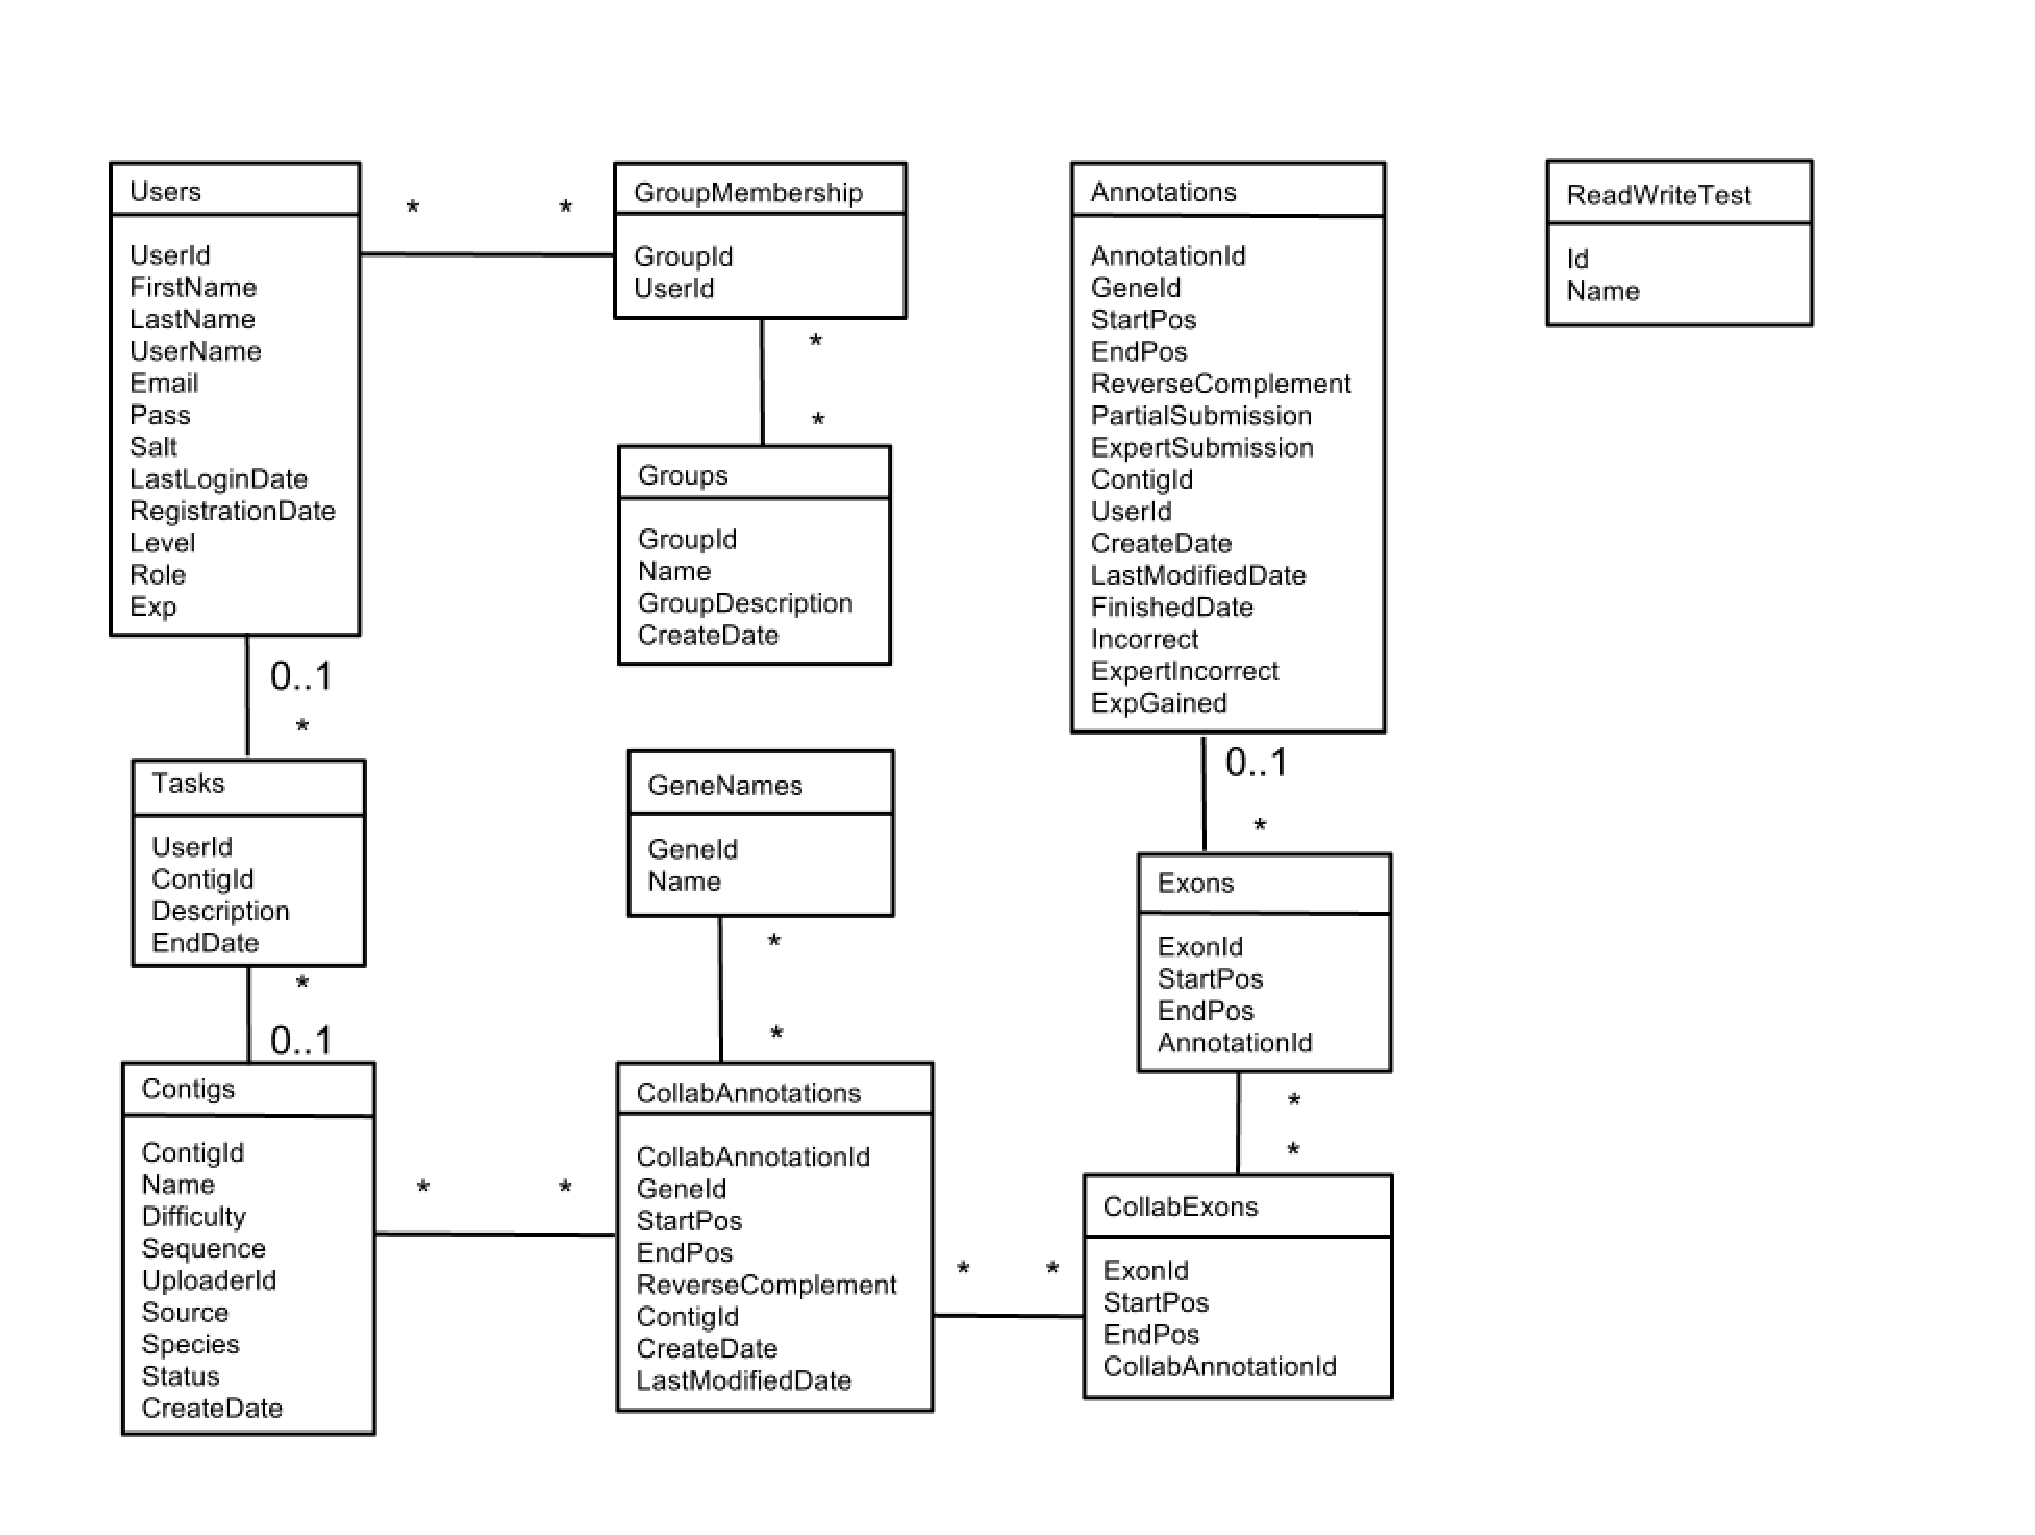
\includegraphics[height=90mm]{SQLDiagram.eps}
	\caption{Entity Relationship diagram for CGAT.}
	\label{fig:SQLDiagram}
\end{figure*}

\begin{figure*}[t]
   \centering
   \subfloat[Contig format]{\label{fig:JSON-contig}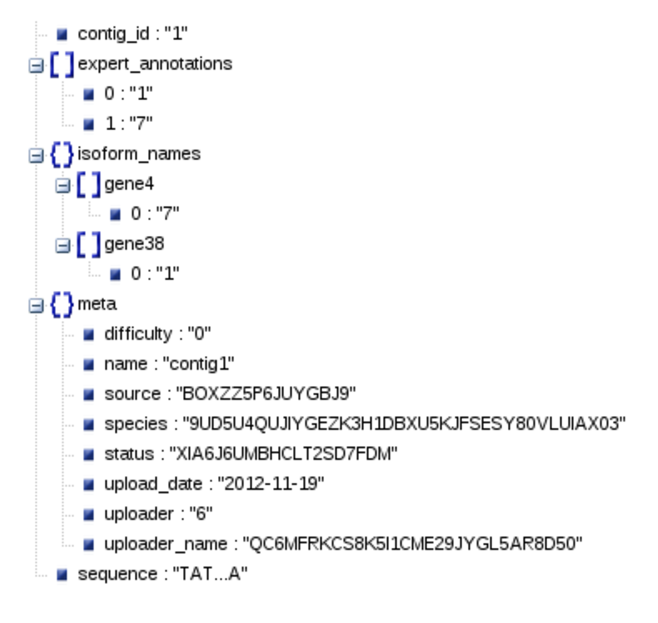
\includegraphics[height=70mm]{contig.eps}}
   \subfloat[Annotation format]{\label{fig:JSON-annotation}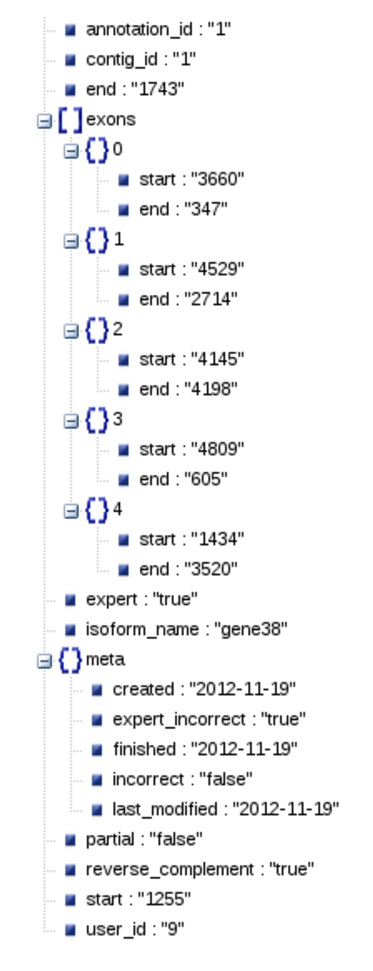
\includegraphics[height=80mm]{annotation.eps}}
   \caption{JSON format for Contigs and Annotations.}
\end{figure*}

\begin{figure*}[t]
   \centering
   \subfloat[User format]{\label{fig:JSON-user}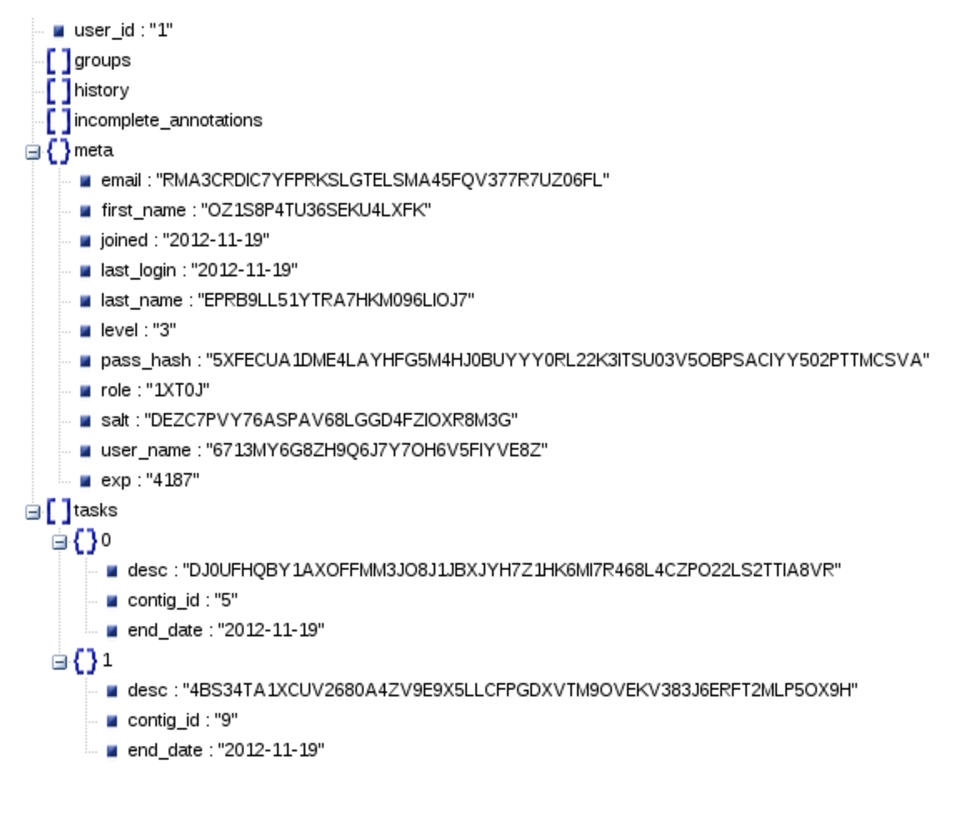
\includegraphics[height=90mm]{user.eps}}
   \subfloat[Group format]{\label{fig:JSON-group}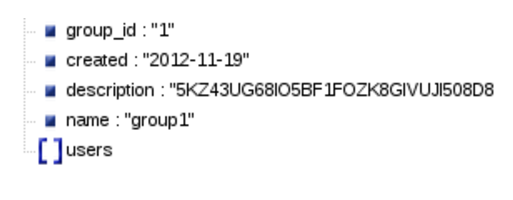
\includegraphics[height=25mm]{group.eps}}
   \caption{JSON format for Users and Groups.}
\end{figure*}

%\begin{figure*}
%  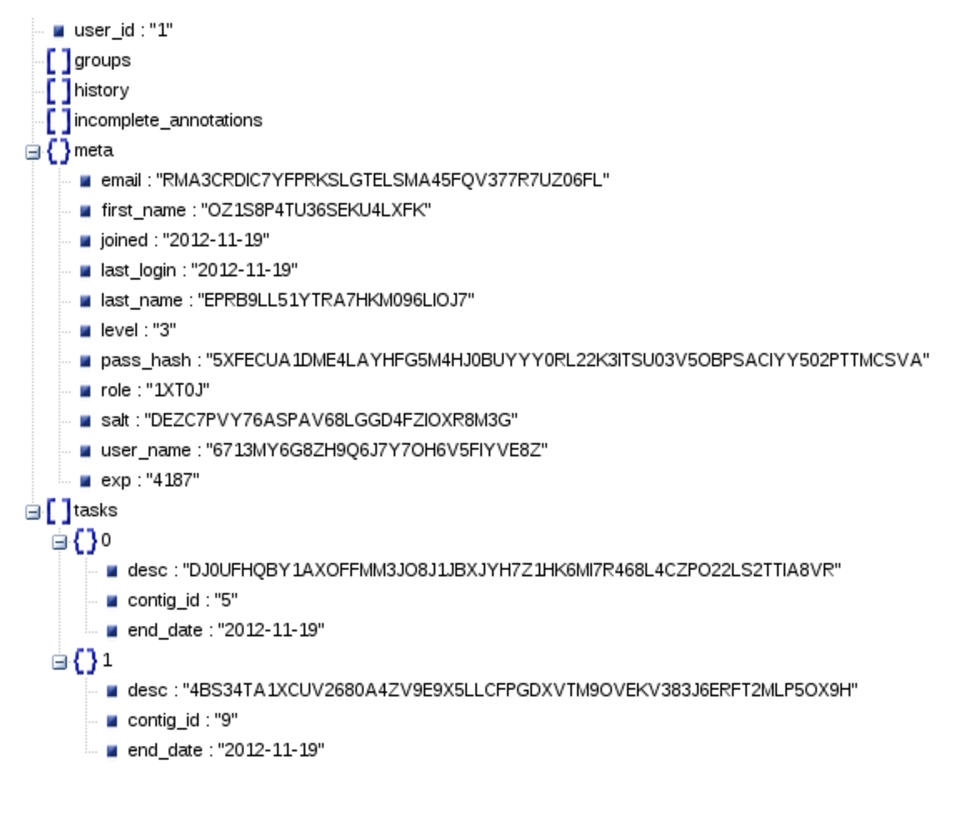
\includegraphics[height=90mm]{user.eps}
%	\caption{The JSON for a user.}
%	\label{fig:JSON-user}
%\end{figure*}
%\begin{figure*}
%  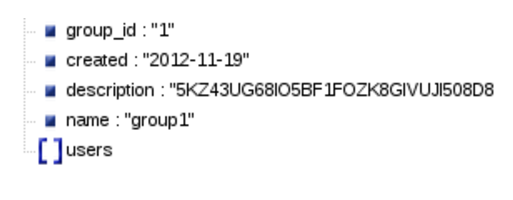
\includegraphics[height=25mm]{group.eps}
%	\caption{The JSON for a group.}
%	\label{fig:JSON-group}
%\end{figure*}
%\begin{figure*}
%  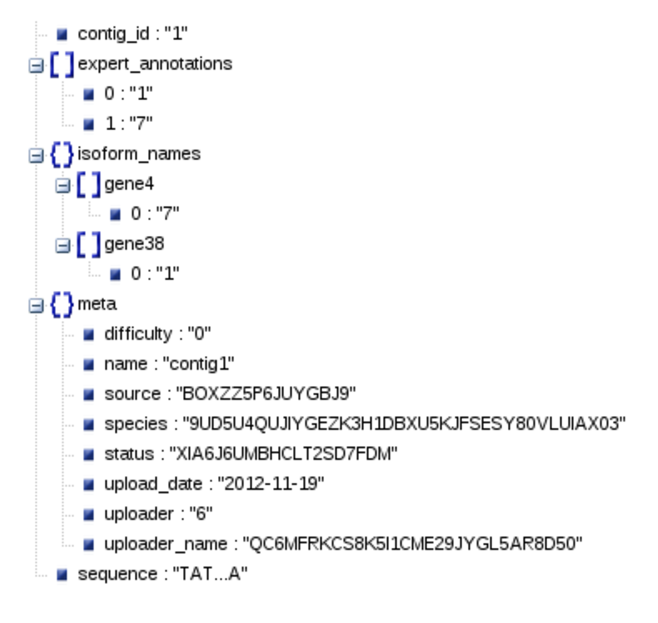
\includegraphics[height=80mm]{contig.eps}
%  \caption{The JSON for a contig.}
%  \label{fig:JSON-contig}
%\end{figure*}
%\begin{figure*}
%  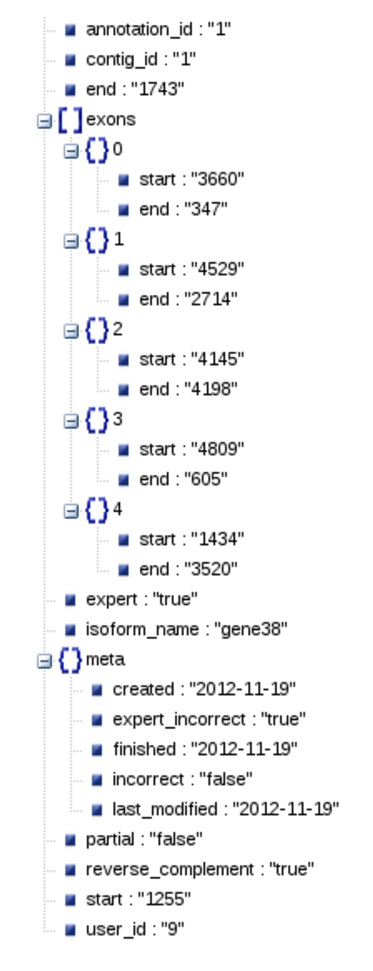
\includegraphics[height=90mm]{annotation.eps}
%	\caption{The JSON for an annotation.}
%	\label{fig:JSON-annotation}
%\end{figure*}

% TODO: Uncomment if we use any refs
% \bibliographystyle{acm}
% \bibliography{refs}

\end{document}
